\section{Formulas and equations}
Please use labels to refer to your equations, like in Eq.~\eqref{eq:T}:
\begin{equation}
  T(s) = \frac{3001 \: (1 + 0.3343s)}{s^3 + 3 s^2 + 3s + 1} \text{.}
  \label{eq:T}
\end{equation}
Equations do not relieve you from the use of punctuation marks. Feel free to align long equations like the next one (without numbering, hence the asterisk)
\begin{align*}
  T(s) &= \frac{\frac{K_i}{m s^2 - K_x} \: K_R \: \frac{1 + s \tau_1}{1 + s \tau_2}}
          {1 + \frac{K_i}{m s^2 - K_x} \: K_R \: \frac{1 + s \tau_1}{1 + s \tau_2}} \\
       &= \frac{K_i K_R (1 + s \tau_1)}{(m s^2 - K_x) (1 + s \tau_2) + K_i K_R (1 + s \tau_1)} \\
       &= \frac{K_i K_R (1 + s \tau_1)}
          {m \tau_2 s^3 + m s^2 + (\tau_1 K_i K_R - \tau_2 K_x) s + K_i K_R - K_x} \\
       &= \frac{K_i K_R \: \frac{1 + s \tau_1}{m \tau_2}}
          {s^3 + \frac{1}{\tau_2} s^2 + \frac{\tau_1 K_i K_R - \tau_2 K_x}{m \tau_2} s 
          + \frac{K_i K_R - K_x}{m \tau_2}} \text{.}
\end{align*} 
If you use indices like $x$ in $A_x$, please define them as text if they are not variables like in $A_\text{Beer}$. Note that $A_{Beer}$ would be wrong. Stick to the notation from~\cite{Sko05} or the lecture notes as far as possible. Matrices and vectors should be bold faced, for example $\mathbf{A}$ or $\mathbf{u}$. Please use the siunitx package for adding SI units to numerical values, example \SI[per-mode=fraction]{5}{\meter\per\second}.

\section{Figures}
Please add figures in a floating figure environment as shown in Fig.~\ref{fig:superC}.
\begin{figure}[htb]
  \centering
  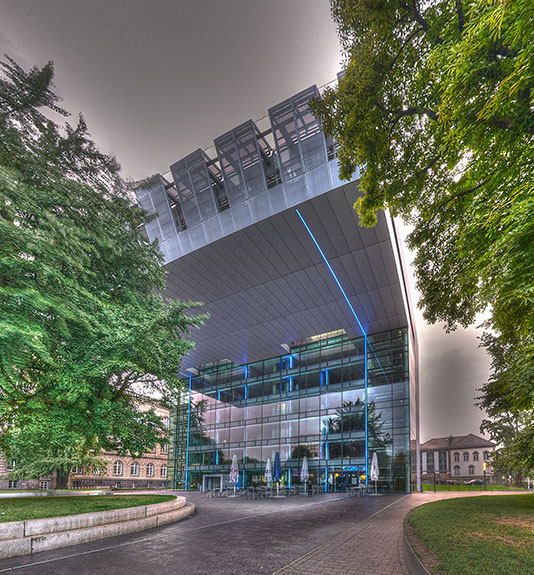
\includegraphics[scale=0.5]{images/superC}
  \caption{Nice picture of the big bus stop.}
  \label{fig:superC}
\end{figure}
Figures should be not wider than the attribute textwidth, starting with a backslash. Please note the full stop at the end of the caption of the figure. And note that the figure floats away, a nice explanation from Wikipedia: Floats are not part of the normal stream of text, but separate entities, positioned in a part of the page to themselves (top, middle, bottom, left, right, or wherever the designer specifies). They always have a caption describing them and they are always numbered so they can be referred to from elsewhere in the text. LaTeX automatically floats Tables and Figures, depending on how much space is left on the page at the point that they are processed. If there is not enough room on the current page, the float is moved to the top of the next page. This can be changed by moving the Table or Figure definition to an earlier or later point in the text, or by adjusting some of the parameters which control automatic floating.
